\section{Observations and models}

\subsection{Selection of observations}
We conduct our survey on 139 images taken by the Cassini Image Sub-System Narrow Angle Camera (ISS-NAC) with the
clear and ultra-violet filters (CL1-UV3). We choose the best possible sample among the 317 images available on the PDS
to get the highest temporal and phase coverage. We kept only images taken with at least one day apart for the main study.
We also kept specific sets of observations made few hours apart to study short term variations.

On average, the selected images are separated by 39 Earth days, \textit{i.e.} 2.5 Titan days (Fig.~\ref{fig:img_sampling}).
Even if our sampling is not evenly distributed, due to orbital constraints and mission schedule, at least 90\% of the selected
images are separated by less than 120 Earth days, \textit{i.e.} 7.5 Titan days. Two main gaps of data can be observed in dataset.
The first between 28 March 2008 and 25 January 2009 (302 Earth days) and 26 November 2010 and 9 September 2011 (286 Earth days).

\begin{figure}[!ht]
\centering
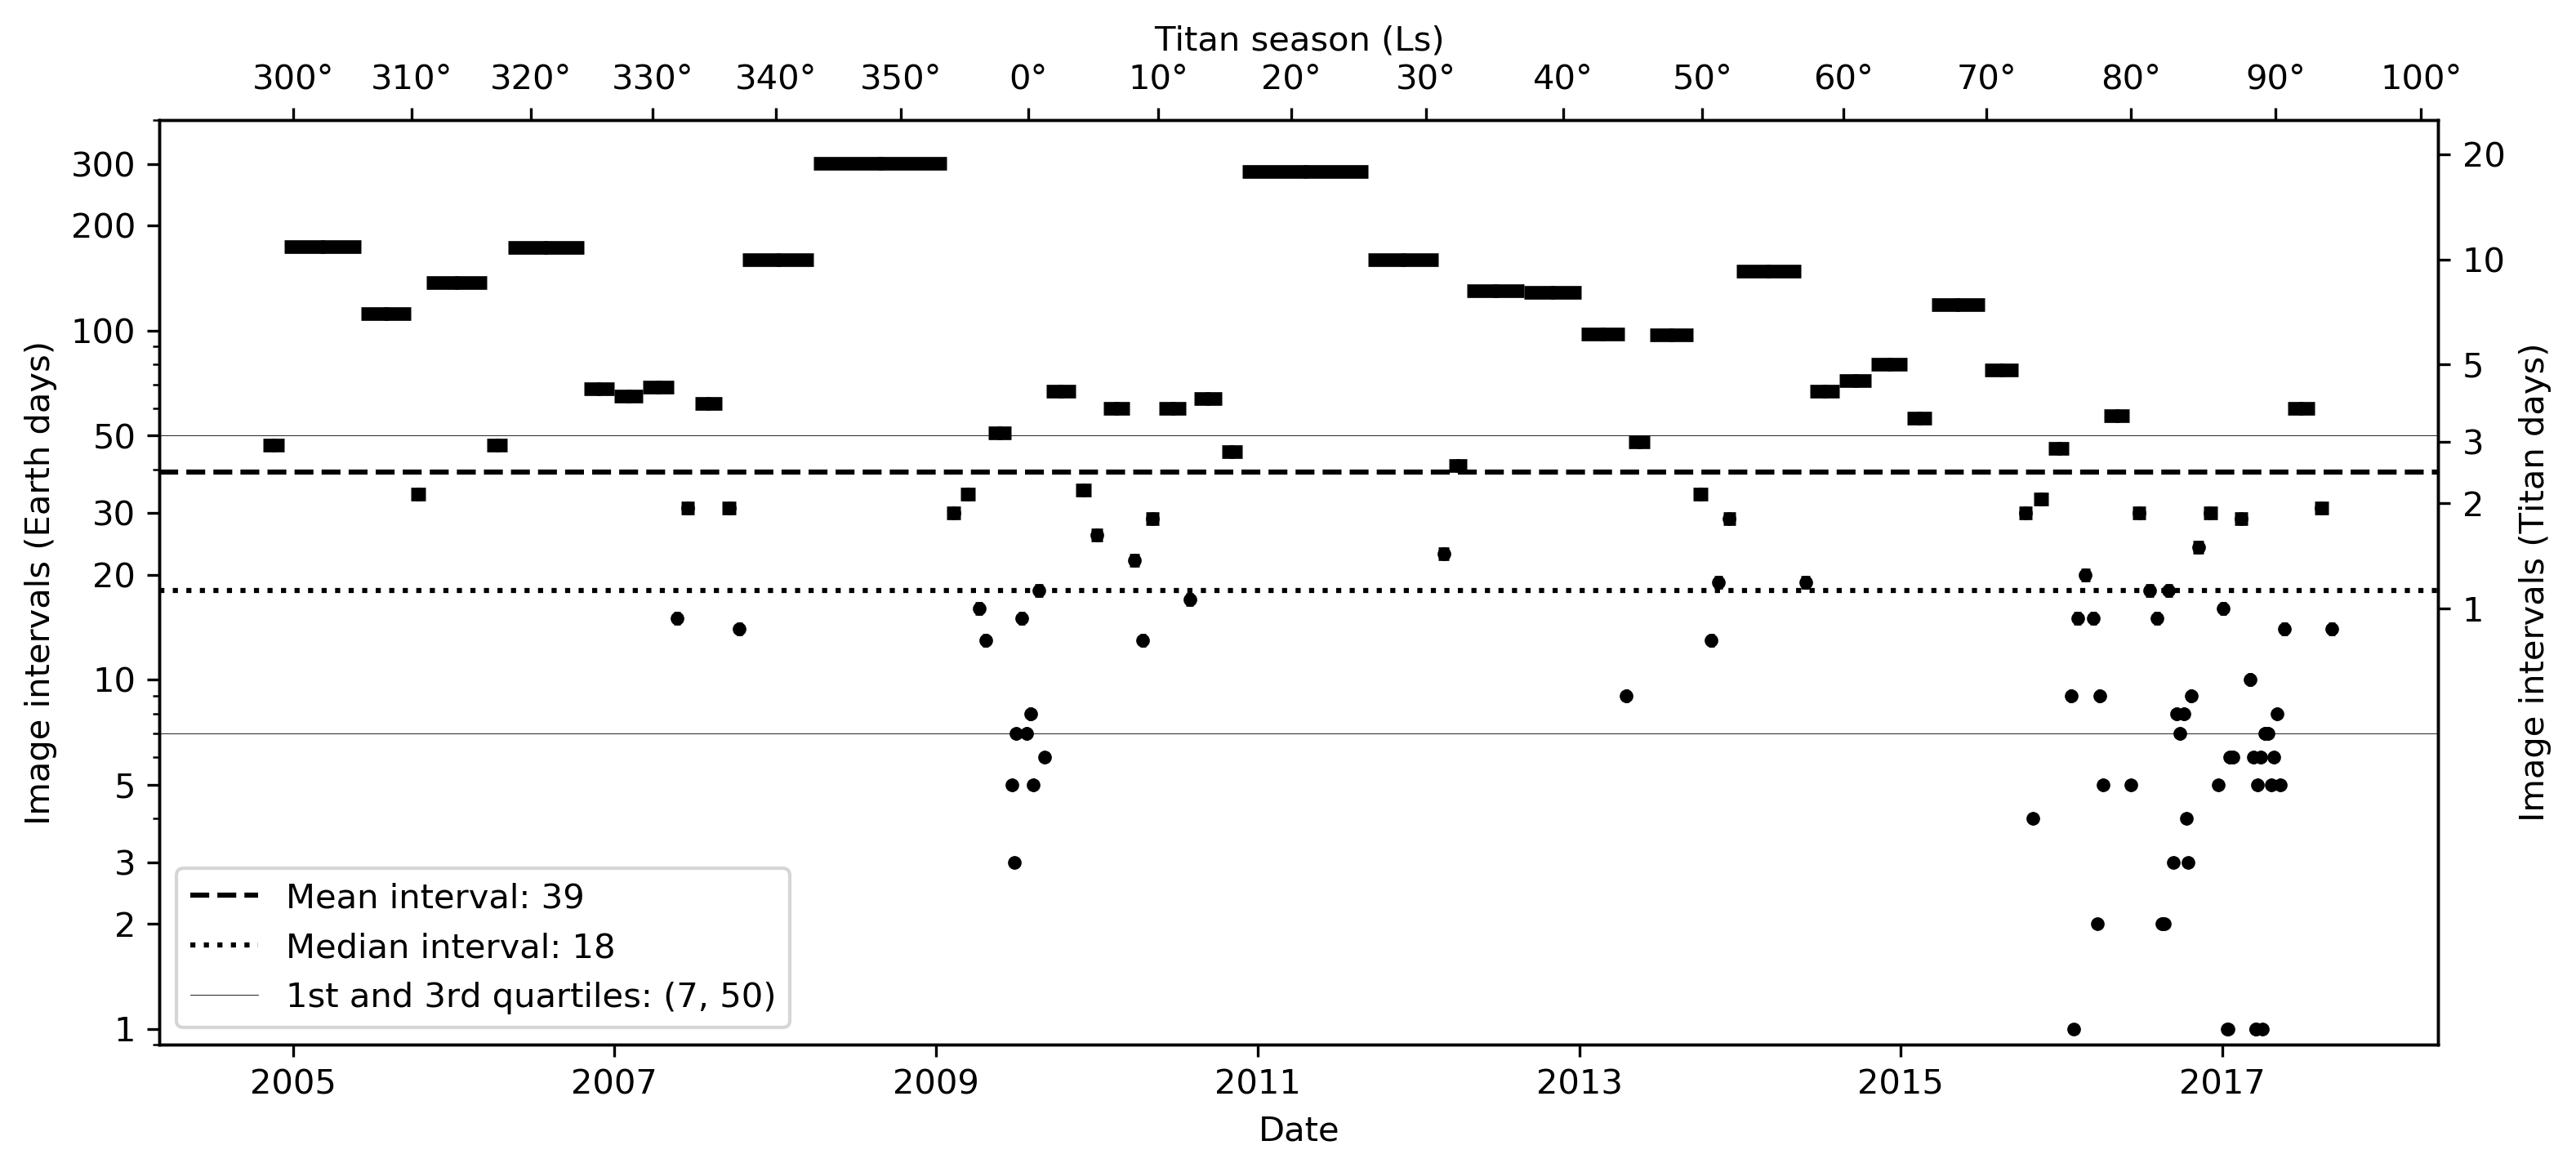
\includegraphics[width=\textwidth]{Fig/IMG_interval.png}
\caption{Image intervals (in Earth and Titan days) between consecutive ISS/NAC CL1-UV3 observations analyzed. On average
an image is sampled every 39 days.}
\label{fig:img_sampling}
\end{figure}

The selected images are calibrated using the CISSCAL routines (v3.8) provided on the Planetary Data System. To improve
the signal to noise ratio on the limb profile, we deconvolved the images with a Poisson Maximum a posteriori method
(PMAP) using the point spread function (PSF) calculated in-flight \citep{West2010}. The image pointing is
initialized with the SPICE kernels \citep{Acton1996}. Since the surface of Titan is not visible in the UV, we improved
the location of Titan center by fitting the limb intensity. Then, we calculated the planetocentric coordinates of each
pixels and their altitude with respect to a mean spherical body with a radius of 2575 km.

Intensity profiles are extracted every \ang{5} on both sides of the limb. Depending on the location of the
latitude of the Sub-Cassini point on the ground, the sampling in latitude is not evenly distributed for each image.
Therefore, the polar latitudes are usually less covered than the equator.
We should also note that the solar illumination changes drastically during the
season between the northern mid-winter to summer, which restricts our ability to see both poles at the same time.


\subsection{Model of scattering at the limb}

To retrieve the haze extinction profiles from the intensity observations, we model the synthetic
radiance factor ($I/F$) with a single scattering ray tracing model in a spherical shell geometry.
The effect of the multiple scattering is accounted as a correction with a factor $\varrho_k\left(z\right)$
applied to the volume scattering along line of sight.
This technique was used successfully several time before \citep[e.g.][]{Rages1983, Rannou1997, Seignovert2017, West2018}.

In the detached layer, the multiple scattering is mainly produced by the light coming from the atmosphere below. To
evaluate $\varrho_k$, the scattering properties of the atmosphere are fixed once for all with a setup that allows to
reproduce the observed intensity of Titan in UV. With a radiative transfer model \citep[SHDOMPP, from ][]{Evans1998}
we have access to the complete radiative source function at each level of the atmosphere. We are then able to compare the
intensity that is scattered in the direction of the observer from the direct sun only and from the direct sun and the diffuse
field coming from below. $\varrho_k$ is defined as the ratio of multiple scattering to single scattering toward the observer
for a given altitude and as a function of the incident and emergent angles. This parameter is pre-computed as a function
altitude, incident and emergent angle and saved in a look-up table \citep[see.][for details]{West2018}.
We find that the multiple scattering increases the scattered intensity at the limb of Titan in UV by a ratio between
1.05 and 1.15, depending on the geometry of the observation.

We discretize the atmosphere in $N=60$ irregular layers of various thickness : $\Delta z =$ 50 km from the
ground to 200 km, $\Delta z =$ 10 km from 300 to 400 km and from 550 to 700 km. Finally, we used
$\Delta z$= 5 km between 400 and 550 km. This grid allows us to take advantage of the spatial resolution
of the ISS NAC camera in the region of interest where is mainly located the DHL.

Finally, we can write the outgoing radiance factor $I/F (z)$ as:

\begin{equation}
I/F (z) = \sum_{i=0}^{n_x-1} \int\limits_{x_k}^{x_{k+1}}
\frac{\left< \varpi P(\Theta) \right>_k} {4}
^{-\left( \tau^i_k\left(z\right) + \tau^e_k\left(z\right) \right)}
\beta_k\left(z\right) \varrho_k\left(z\right) d{x}
\label{eq:west2017_sup_limb}
\end{equation}

where the summation is performed on the $n_x-1$ segments defined by the intersections of the line of sight and the
spherical shells boundaries. The impact factor $z$ (the lowest altitude reached by the line of sight) is given by the
bottom of the $n^\mathrm{th}$ layer crossed. Therefore, each layer of the atmosphere is crossed twice. $x$ is the
abscissa along the line of sight. $\tau^i_k$ and $\tau^e_k$ are the opacities along the incident and emergent paths.
$\left< \varpi P(\Theta)\right>_k$ is the average of the product between the single scattering and the phase function
at the scattering angle of the observation $\Theta$ for the layer crossed on $x_k$.  $\beta_k(z)$ is the local
extinction at the altitude $z$. Here, the altitude $z(x)$ is the local altitude at point of abscissa $x$ along the
line of sight.


\subsection{Retrieval method}

Based on our previous works \citep{Seignovert2017, West2018}, we make the assumption that the optical properties
$\left<\varpi P(\Theta)\right>_k$ of the aerosols are constant in the upper part of Titan's atmosphere. This allows
us to focus our study only on the retrieval of the extinction along the line of sight.
% FIXME: We will verify that this assumption is reasonable compared to the dynamical variability observed along the season.
In our model, the $I/F (z)$ intensity profiles only depend on the set haze extinction profile $\beta(z)$ and the viewing
geometry of the observation (incidence, emergence and phase angles). We assume no horizontal inhomogeneity in the atmosphere
properties along the line of sight \citep{Seignovert2017}. We retrieve a set of extinction values $\beta_i$ (composing
the vector ${\beta}$), with $i$ the indices of the layers, that matches the values of the radiance factor, $I/F_i$
(composing the vector $I/F$).

From the Eq. (\ref{eq:west2017_sup_limb}), it is possible to cast the scattered intensity $I/F_i$, as a function of
the extinction $\beta_j$ with $j \le i$. This forms a non-linear triangular system. To find the vector $\beta$, we
have to solve the formal equation:

\begin{equation}
    I/F = G(\beta)
\end{equation}

where the ${G}$ is a nonlinear function which depends on the values $\beta_i$ and on the viewing geometry of the observation.

We could solve this system with a standard onion peeling technique.
However, we observed a quick propagation of error on the retrieved $\beta_j$ at a given level, by the all the errors from the
layers above ($\beta_i$).
Instead, we decided to solve the system by minimizing globally the difference between the modelled $I/F$ and the observations
using a Levenberg-Marquardt minimization. Therefore, we obtain simultaneously all the $\beta_i$ at once.
Moreover, the tangential opacity along a line of sight ($\tau_{los}$) is consider opaque when it value reach 3.
Beyond this threshold, we do not retrieve the value of $\beta$.
An example of inversion is presented in the figure~\ref{fig:model_uncertainties}.

\begin{figure}[!ht]
    \centering
    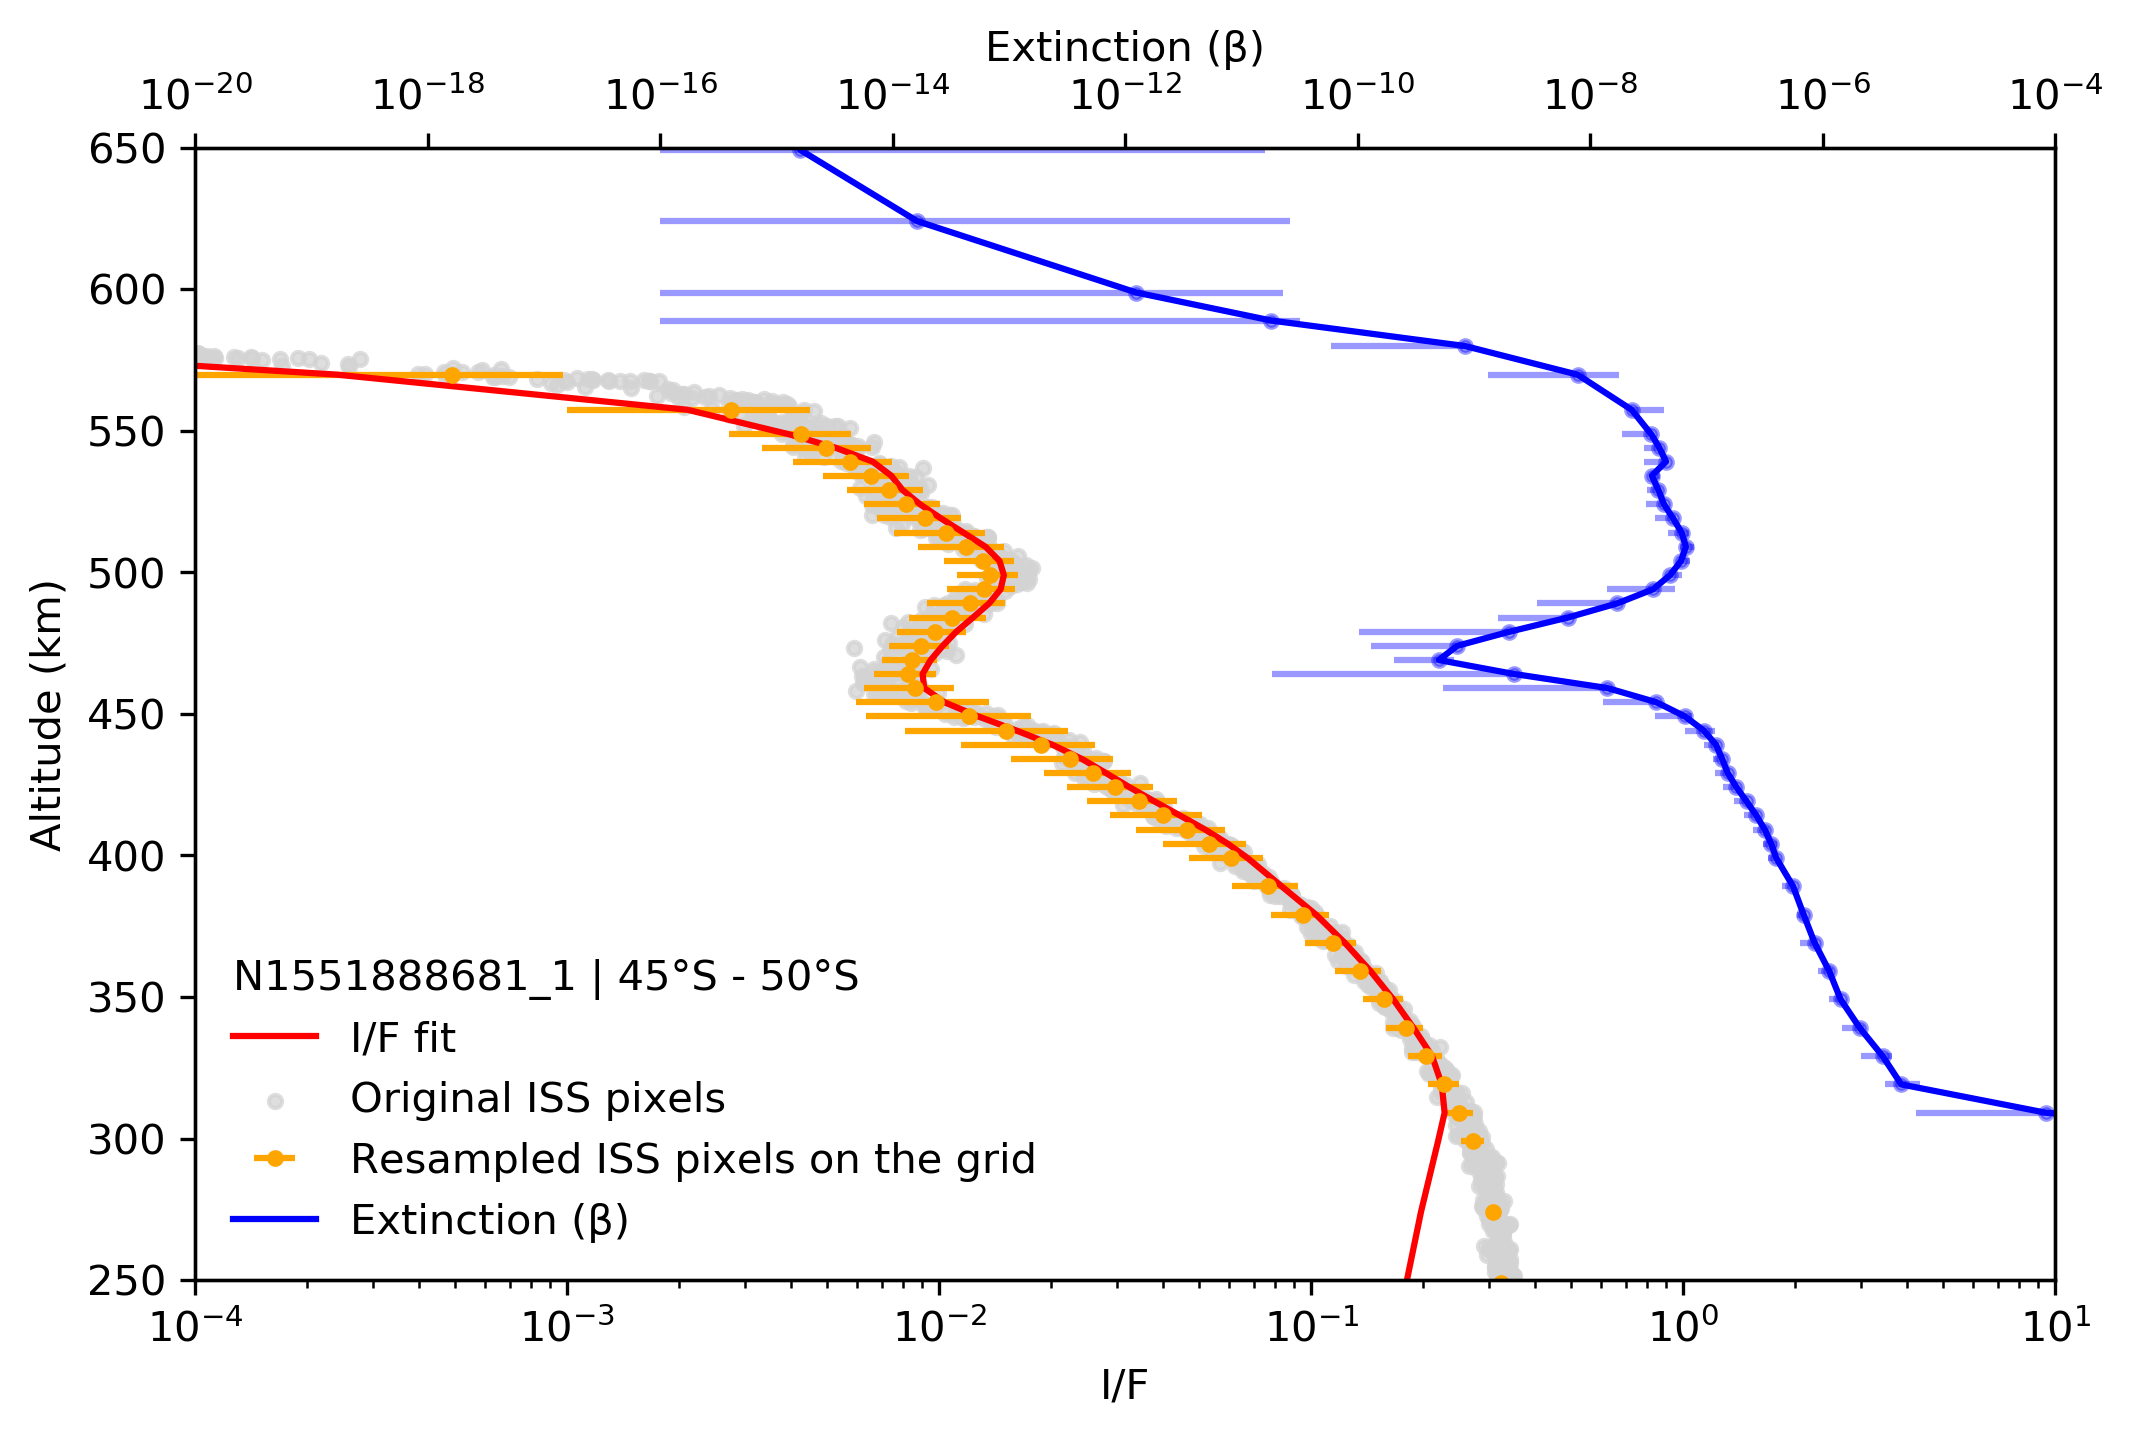
\includegraphics[width=\textwidth]{Fig/Model_uncertainties.png}
    \caption{$I/F$ intensity profile extracted on the image \textbf{N1551888681\_1} at the photometric
             equator ([\ang{45}S, \ang{50}S] and [\ang{76}W, \ang{79}W]). The original ISS pixels
             are resampled on the grid before the inversion. The uncertainties on the retrieved
             extinction profile $\beta$ is calculated to match the $1 \sigma$ dispersion of the
             $I/F$ pixels. We can see that the model can explain the observation down to 300 km.
             The uncertainties increase rapidly when the intensity observed ($I/F$) is close
             to the noise level ($3\cdot10^{-3}$).}
    \label{fig:model_uncertainties}
\end{figure}
